\documentclass[a2paper]{article}

\usepackage{siunitx}
\usepackage{tikz}
\usetikzlibrary{arrows}
\usepackage{amsmath}
\usepackage{geometry}
% \usepackage{showframe}

\geometry{a2paper,margin=0.5in}
\pagestyle{empty}

\newdimen\gpdashlength


\begin{document}
\thispagestyle{empty}

\begin{figure}[h!]
\begin{tikzpicture}
\pgfsetlinewidth{2pt}
\gpdashlength=0.5\pgflinewidth
\tikzset{gp path/.style={dash pattern=on 7.5\gpdashlength off 
7.5\gpdashlength}}

\node[anchor=south west,inner sep=0] at (0.2,-5.0) 
{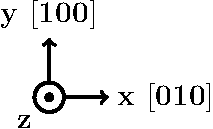
\includegraphics[width=0.30\textwidth]{arrows1}};
\node[anchor=south west,inner sep=0] at (0.2,0.0)  
{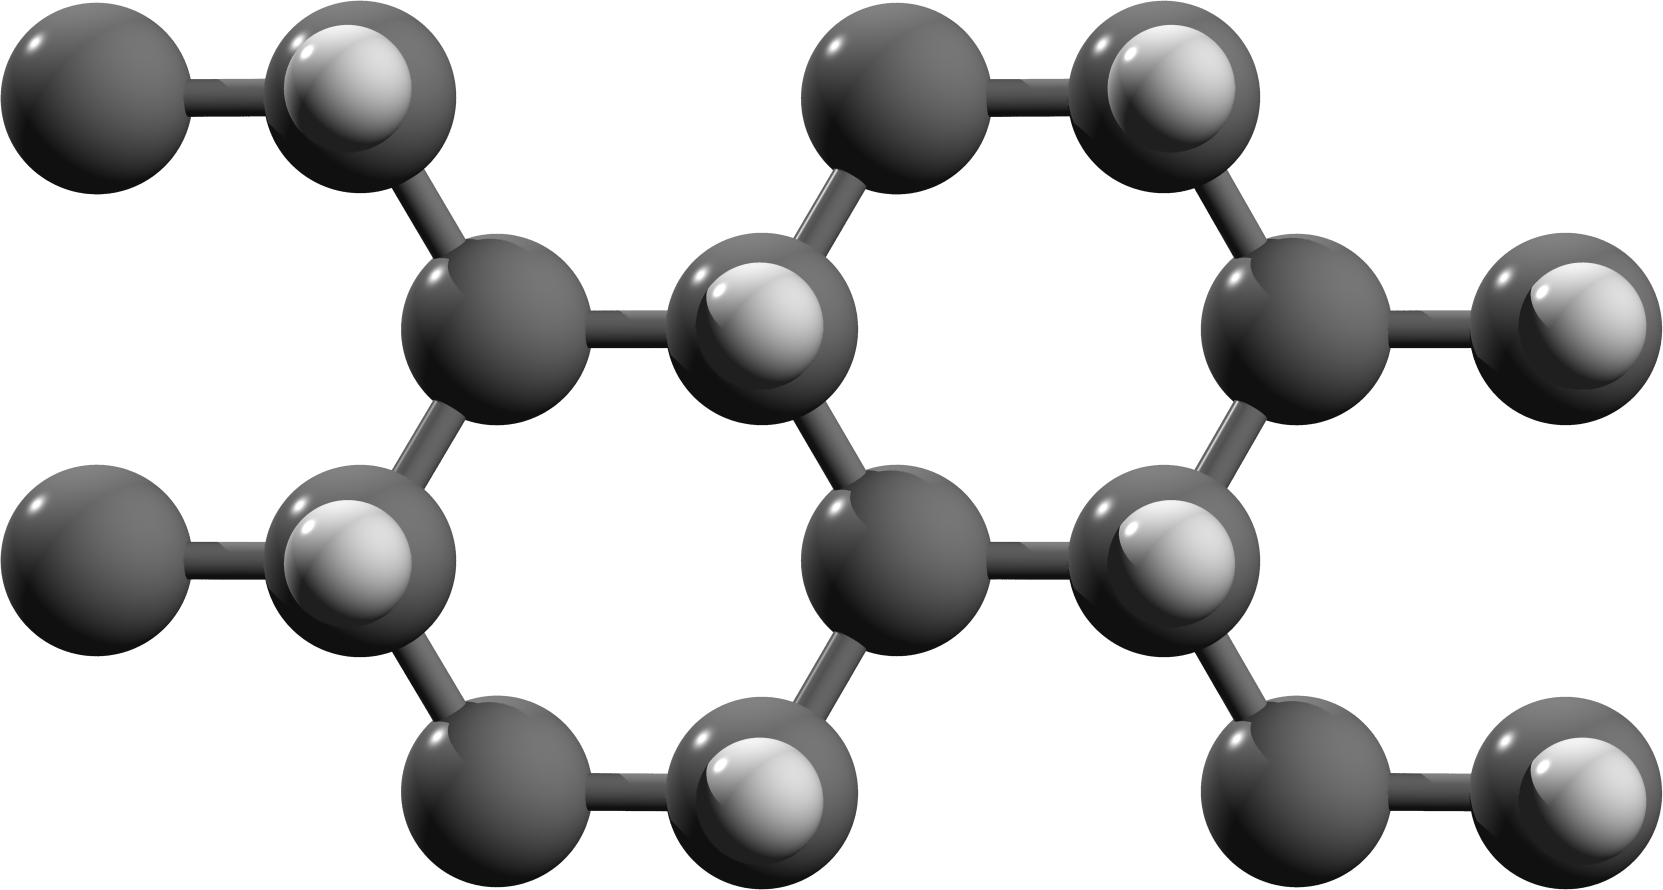
\includegraphics[width=\textwidth]{up1}};
\draw [line width=2.00mm, red, -> ] (8.50,8.00) -- (18.50,13.50) 
node [right] {};
\draw [line width=2.00mm, red, -> ] (8.50,8.00) -- (18.50,02.00) 
node [right] {};
\draw [line width=2.00mm, red, dashed ] (18.50,13.50) -- (28.50,8.00) 
node [right] {};
\draw [line width=2.00mm, red, dashed ] (18.50,02.00) -- (28.50,8.00) 
node [right] {};
\node[anchor=south west,inner sep=0] at (0.2,-20.0) 
{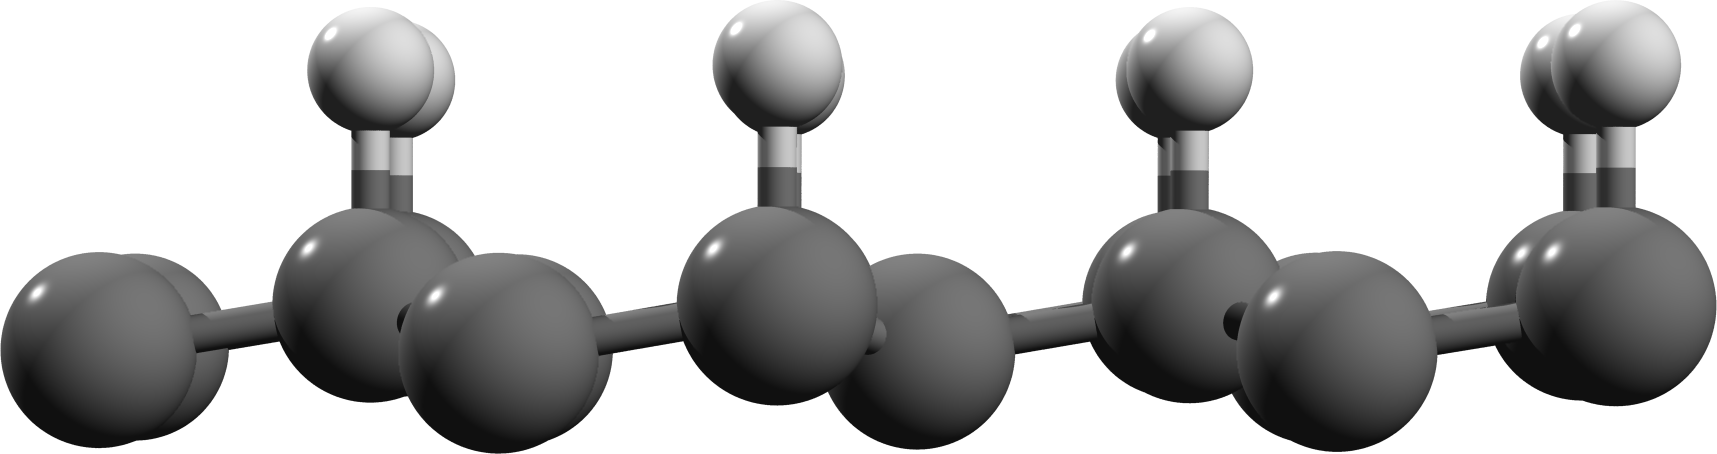
\includegraphics[width=\textwidth]{up2}};
\node[anchor=south west,inner sep=0] at (0.2,-34.0) 
{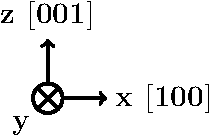
\includegraphics[width=0.30\textwidth]{arrows2}};
\end{tikzpicture}
\end{figure}


\end{document}
